% -*- coding: UTF-8 -*-
% vim: autoindent expandtab tabstop=4 sw=4 sts=4 filetype=tex
% chktex-file 27 - disable warning about missing include files
% chktex-file 36 - disable put space in front of parentheses warning

\begin{titlepage}

    % BFH-Logo absolute placed at (28,12) on A4 and picture (16:9 or 15cm x 8.5cm)
    % Actually not a realy satisfactory solution but working.
    %---------------------------------------------------------------------------
    \setlength{\unitlength}{1mm}
    
\includegraphics[scale=1.0]{img/BFH_Logo_B}

    \begin{picture}(150,2)
        \put(0,0){\color{bfhgrey}\rule{150mm}{2mm}}
    \end{picture}

    \begin{figure}[H]
        \hspace*{0.25cm}
        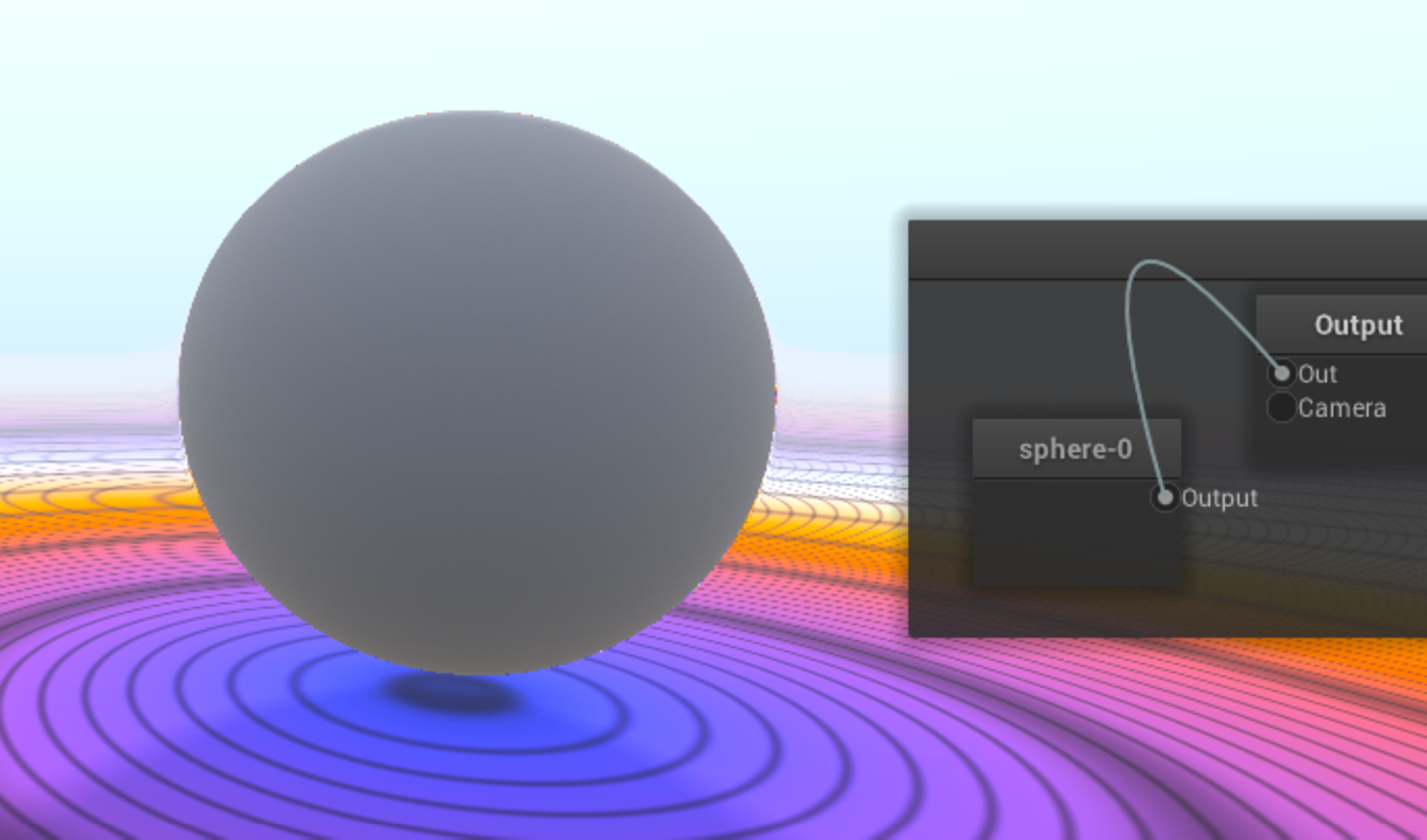
\includegraphics{img/logo.pdf}
    \end{figure}

    \begin{picture}(150,2)
        \put(0,0){\color{bfhgrey}\rule{150mm}{2mm}}
    \end{picture}

    \begin{flushleft}
        \fontsize{26pt}{28pt}\selectfont
        \titel{}\\
        \vspace{3mm}
        \textbf{A visual animation system} \\
        \vspace{6mm}
        \fontsize{14pt}{16pt}\selectfont
        \textbf{MTE7102: Projektarbeit 2} \\
        \vspace{3mm}

        \fontsize{10pt}{17pt}\selectfont
        \begin{tabbing}
        xxxxxxxxxxxxxxx   \= xxxxxxxxxxxxxxxxxxxxxxxxxxxxxxxxxxxxxxxxxxxxxxx \kill
        Studiengang:      \> Informatik                                         \\
        Autor:            \> Sven Osterwalder\protect\footnotemark[1]{}         \\
        Betreuer:         \> Prof.~Claude Fuhrer\protect\footnotemark[2]{} \\
        Datum:            \> \vhCurrentDate{}\\
        Version:          \> \vhCurrentVersion\\
        \end{tabbing}
    \end{flushleft}
    \footnotetext[1]{sven.osterwalder@students.bfh.ch}
    \footnotetext[2]{claude.fuhrer@bfh.ch}

    \vfill
    
\includegraphics[height=\baselineskip]{img/by-sa}\\ \small{\sffamily{Licensed under the Creative Commons Attribution-ShareAlike 3.0 License}}

    \thispagestyle{titlepageStyle}

\end{titlepage}
